% Created 2012-09-09 Sun 17:22
\documentclass[11pt]{article}
\usepackage[utf8]{inputenc}
\usepackage{fixltx2e}
\usepackage{url}
\usepackage{graphicx}
\usepackage{minted}
\usepackage{color}
\usepackage{longtable}
\usepackage{float}
\usepackage{wrapfig}
\usepackage{soul}
\usepackage{textcomp}
\usepackage{amsmath}
\usepackage{marvosym}
\usepackage{wasysym}
\usepackage{latexsym}
\usepackage{amssymb}
\usepackage[linktocpage,
  pdfstartview=FitH,
  colorlinks,
  linkcolor=blue,
  anchorcolor=blue,
  citecolor=blue,
  filecolor=blue,
  menucolor=blue,
  urlcolor=blue]{hyperref}
\usepackage{attachfile}
\tolerance=1000
\providecommand{\alert}[1]{\textbf{#1}}

\title{HOMEWORK 1 - Due 9/6/2012}
\author{Zhongnan Xu}
\date{9/6/12 Thursday}
\hypersetup{
  pdfkeywords={},
  pdfsubject={},
  pdfcreator={Emacs Org-mode version 7.8.11}}

\begin{document}

\maketitle

\setcounter{tocdepth}{3}
\tableofcontents
\vspace*{1cm}

\section{Signup for an account at gitHub.}
\label{sec-1}

Print your username here: zhongnanxu (note, I've changed it from my
previous `xuzho' one for consistency)

Set yourself up to \href{http://www.quora.com/GitHub/What-does-it-mean-to-watch-in-GitHub}{watch}
\href{https://github.com/jkitchin/dft-course}{https://github.com/jkitchin/dft-course} and
\href{https://github.com/jkitchin/dft-book}{https://github.com/jkitchin/dft-book}.
\section{Read Chapter 1 in the text book.}
\label{sec-2}

You do not need to write anything. Just do it.
\section{Read Section 5 (Molecules) in dft-book.}
\label{sec-3}

As part of this assignment, please turn in a pdf copy of dft-book that has been annotated by sticky notes using Adobe Acrobat Reader (you should be able to type Ctrl-6 to get a sticky note while the pdf is open, and then you can move it where you want and type text in it.). Please note any typos, places that are confusing, etc\ldots{}

Please see pdf file in the hw-1 folder
\section{Data fitting.}
\label{sec-4}

Fit a cubic polynomial to this set of data and estimate the lattice 
constant that minimizes the total energy. Prepare a figure that shows 
the data, your fit and your estimated minimum. Hints: \texttt{numpy.polyfit},
\texttt{numpy.polyder}, \texttt{numpy.roots}, \texttt{numpy.linspace}, \texttt{numpy.polyval} will 
all help you do this easily.


\begin{center}
\begin{tabular}{rr}
 lattice constant ($\AA$)  &  Total Energy (eV)  \\
\hline
                      3.5  &          -3.649238  \\
                     3.55  &          -3.696204  \\
                      3.6  &          -3.719946  \\
                     3.65  &          -3.723951  \\
                      3.7  &          -3.711284  \\
                     3.75  &           -3.68426  \\
\end{tabular}
\end{center}



Code

\begin{minted}[frame=lines,fontsize=\scriptsize,linenos]{python}
import numpy as np
import matplotlib.pyplot as plt

lats, energies = zip(*table)
coeffs = np.polyfit(lats, energies, 3)
ders = np.polyder(coeffs)
roots = np.roots(ders)
# We now need to see what the roots are and pick the sensible one
print 'The two roots are {0:1.3f} and {1:1.3f}'.format(roots[0], roots[1])
print 'Therefore, {0:1.3f} is the minimum lattice constant'.format(roots[1])
lats_func = np.linspace(3.45, 3.80)
energies_func = np.polyval(coeffs, lats_func)

fig = plt.figure(1, (5, 4))
ax = fig.add_subplot(111)
ax.plot(lats, energies, marker='o', linestyle='None', color='k',
        label='Experimental values')
ax.plot(lats_func, energies_func, marker='None', linestyle='-', color='r',
        label='Fitted values')
ax.set_xlabel('Lattice constant ($\AA$)', size='large')
ax.set_ylabel('Total Energy (eV)', size='large')
ax.legend(prop={'size':'medium'})
fig.tight_layout()
plt.show()
\end{minted}

Output
\begin{verbatim}
 The two roots are 4.233 and 3.636
 Therefore, 3.636 is the minimum lattice constant
\end{verbatim}

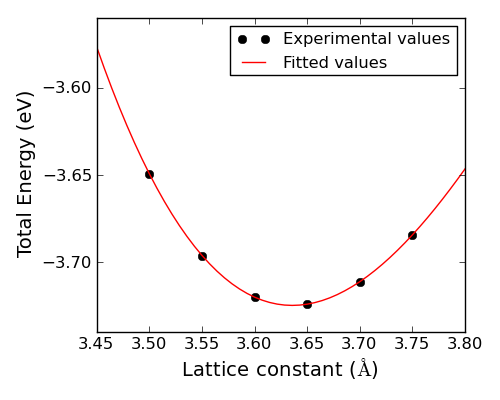
\includegraphics[width=.9\linewidth]{./hw1_data-fitting.png}
\section{Nonlinear algebra}
\label{sec-5}

Solve this equation: $\sin(x^2) = 0.5$ for $x$. Prepare a plot of the function
and show where your solution is. Hint: \texttt{scipy.optimize.fsolve}

Code

\begin{minted}[frame=lines,fontsize=\scriptsize,linenos]{python}
import numpy as np
from scipy.optimize import fsolve
import matplotlib.pyplot as plt

def func(x):
    return np.sin(x**2) - 0.5
print 'The answer is {0:1.3f}'.format(fsolve(func, np.pi)[0])
fig = plt.figure(1, (5, 4))
ax = fig.add_subplot(111)
x = np.linspace(0, 2 * np.pi)
y = func(x) + 0.5
ax.plot(x, y, marker='None', color='b', label='$sin(x^2)$')
ax.plot(2.983, np.sin(2.983**2), marker='o', color='r', label='My solution')
ax.set_xlabel('x')
ax.set_ylabel('y')
ax.set_xlim((0, 2 * np.pi))
ax.legend(prop={'size':'medium'}, loc=3)
fig.tight_layout()
plt.show()
\end{minted}

Output
\begin{verbatim}
 The answer is 2.983
\end{verbatim}

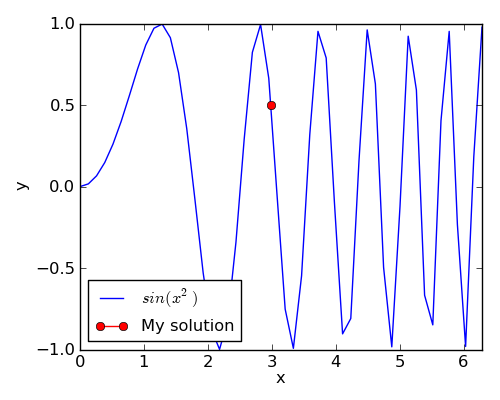
\includegraphics[width=.9\linewidth]{./hw1_linear-algebra.png}
\section{Linear algebra}
\label{sec-6}

Solve these equations using python and linear algebra:

\begin{eqnarray}
a0 - 3 a1 + 9 a2 - 27 a3 = -2 \\
a0 - a1 + a2 - a3 = 2 \\
a0 + a1 + a2 + a3 = 5 \\
a0 + 2a1 + 4 a2 + 8 a3 = 1
\end{eqnarray}

Use linear algebra to verify your solution. Hint: see \texttt{numpy.linalg}, \texttt{numpy.dot}.

Code

\begin{minted}[frame=lines,fontsize=\scriptsize,linenos]{python}
import numpy as np
# This can be solved with matrix algebra, Ax = B
a = np.array([[1, -3, 9, -27],
             [1, -1, 1, -1],
             [1, 1, 1, 1],
             [1, 2, 4, 8]])
b = np.array([-2, 2, 5, 1])
x = np.linalg.solve(a, b)
print 'The answer is'
print 'a0={0:1.3f}'.format(x[0])
print 'a1={0:1.3f}'.format(x[1])
print 'a2={0:1.3f}'.format(x[2])
print 'a3={0:1.3f}'.format(x[3])
# Check that the solution is correct by performing a 
# A dot x operation
print np.dot(a, x)
\end{minted}

Output
\begin{verbatim}
 The answer is
 a0=4.650
 a1=1.842
 a2=-1.150
 a3=-0.342
 [-2.  2.  5.  1.]
\end{verbatim}

\end{document}
